\setAuthor{Taavet Kalda}
\setRound{lahtine}
\setYear{2023}
\setNumber{G 9}
\setDifficulty{9}
\setTopic{TODO}

\prob{Klots ja silinder}
\begin{wrapfigure}[8]{r}{0.4\linewidth}
    \vspace{-25pt}
    \begin{center}
        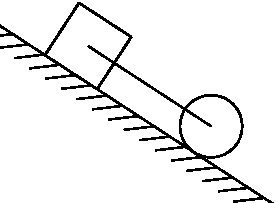
\includegraphics[width=\linewidth]{2023-lahg-09-yl.pdf}
    \end{center}
\end{wrapfigure}
Anul on samasuguse läbimõõdu ja massiga pikk silinder ja klots. Ta lasi silindril mäenõlvast alla veereda ning mõõtis ajaks $t_1 = \SI{5}{\second}$. Seejärel lasi ta klotsil alla libiseda ning sai ajaks $t_2 = \SI{7}{\second}$. Kui palju kuluks silindril ja klotsil mäest alla jõudmiseks, kui need joonisel näidatud moel liigesega ühendada? Võib eeldada, et mäenõlv on ühtlase kaldenurgaga, hõõrdejõud kõikide pindade vahel on konstantne, silinder veereb alati libisemata ning et igas stenaariumis läbisid objektid sama vahemaa. Silindri inertsimoment on $I=mR^2/2$, kus $m$ on silindri mass ja $R$ selle raadius. Õhutakistusega mitte arvestada.









\newcommand{\magnetvali}{
    \begin{tikzpicture}[scale=0.70]
        \draw (-4,0) -- (4,0);
        \draw (0,-4) -- (0,4);

        \draw[thick,->] (0,2) node [anchor = east] {$(0,h)$}
                            -- ++(60:1.6)
                            node [midway, anchor = west] {$\Vec{v}$};
        \draw (0,2) -- ++ (60:1) node [midway, anchor = south east, xshift = 6] {$\alpha$}
            arc (60:90:1);

        \draw (-2,2) circle (0.25) node[above, anchor = south, yshift = 5] {$B_1$};
        \filldraw (-2,2) circle (0.05);
        
        \draw (2,-2) circle (0.25) node[above, anchor = south, yshift = 5] {$B_1$};
        \filldraw (2,-2) circle (0.05);

        \draw (2,2) circle (0.25) node[above, anchor = south, yshift = 5] {$B_2$};
        \draw (2.25,2) -- (1.75,2);
        \draw (2,1.75) -- (2,2.25);

        \draw (-2,-2) circle (0.25) node[above, anchor = south, yshift = 5] {$B_2$};
        \draw (-2.25,-2) -- (-1.75,-2);
        \draw (-2,-1.75) -- (-2,-2.25);
        
    \end{tikzpicture}
} 

\setlength{\columnsep}{20pt}

\hint

\solu
Olgu nõlva kaldenurk $\alpha$ ning hõõrdetegur $\mu$.

Kuna silinder veeres libisemata, asus selle pöörlemiskese silindri ja mäenõlva kontaktpunktis. Vaatleme jõumomentide tasakaalu selle punkti suhtes. Kui silindri nurkkiirendus on $\epsilon$, siis
\[
I'\epsilon = mgR\sin\alpha,
\]
kus $I' = mR^2/2 + mR^2 = 3/2 mR^2$ on silindri inertsimoment kontaktpuntki läbiva telje suhtes (kasutades Steineri teoreemi). Silindri kiirendus on seega
\[
a_1 = R\epsilon = \frac{mR^2}{I'} \sin\alpha = \frac{2}{3}g\sin\alpha.
\]

Klotsi kiirendus allamäge takistab hõõrdejõud $mg\cos\alpha \mu$ ning kiirendab raskusjõud $mg\sin\alpha$. Klotsi kiirendus on seega
\[
a_2 = g\sin\alpha\mu - g\cos\alpha\mu.
\]
Peale silindri ja klotsi ühendamist hakkavad nad ühtse kehana mäest alla kiirenema kiirendusega $a_3$. Kui liigese pinge on $T$, siis silindrile mõjuvad jõud on raskuskiirendus, liigese pinge ning hõõrdejõu ja toereaktsiooni resultant. Kuna silinder ei libise, võime silindri jõumomentide tasakaalu jälle mäenõlva kontaktpunkti suhtes vaadelda (sest siis $a_3 = \epsilon / R$):
\[
I'\epsilon = mgR\sin\alpha + TR = I'\frac{a_3}{R}.
\]
Liigese pinge on seega
\[
T = \frac{3}{2}ma_3 - mg\sin\alpha.
\]
Klotsile mõjuvad sarnaselt liigese pinge, raskuskiirendus ning hõõrdejõu ja toereaktsiooni resultant. Mäenõlvaga paralleelne jõudude tasakaal esitub kujul
\[
ma_3 = mg\sin\alpha - T - mg\cos\alpha\mu = 2mg\sin\alpha - \frac{3}{2}ma_3 - mg\cos\alpha\mu.
\]
Seega,
\[
a_3 = \frac{4}{5}g\sin\alpha - \frac{2}{5}g\cos\alpha\mu.
\]
Näeme, et
\[
a_3 = \frac{2}{5}a_2 + \frac{3}{5}a_1.
\]
Ei tule suure üllatusena et tegu on kaalutud keskmisega, kus kiirendus on esimese ja teise stsenaariumite kiirenduste vahel.

Kui mäenõlva pikkus on $L$, siis kehtib $L = at^2/2$, st
\begin{align*}
t_3 &= \sqrt{\frac{2L}{a_3}} = \sqrt{\frac{2L}{\frac{2}{5}a_2 + \frac{3}{5}a_1}} = \sqrt{\frac{2L}{\frac{2}{5}\frac{2L}{t_2^2} + \frac{3}{5}\frac{2L}{t_1^2}}}\\
&= \sqrt{\frac{5}{2t_1^2+3t_2^2}}t_1t_2 = \SI{5.6}{s}.
\end{align*}
\probend